%-----------------------------------------------------------------------------%
\chapter{\babEmpat}
\label{bab:4}

\section{Desain Sistem}

\begin{figure}
    \centering
    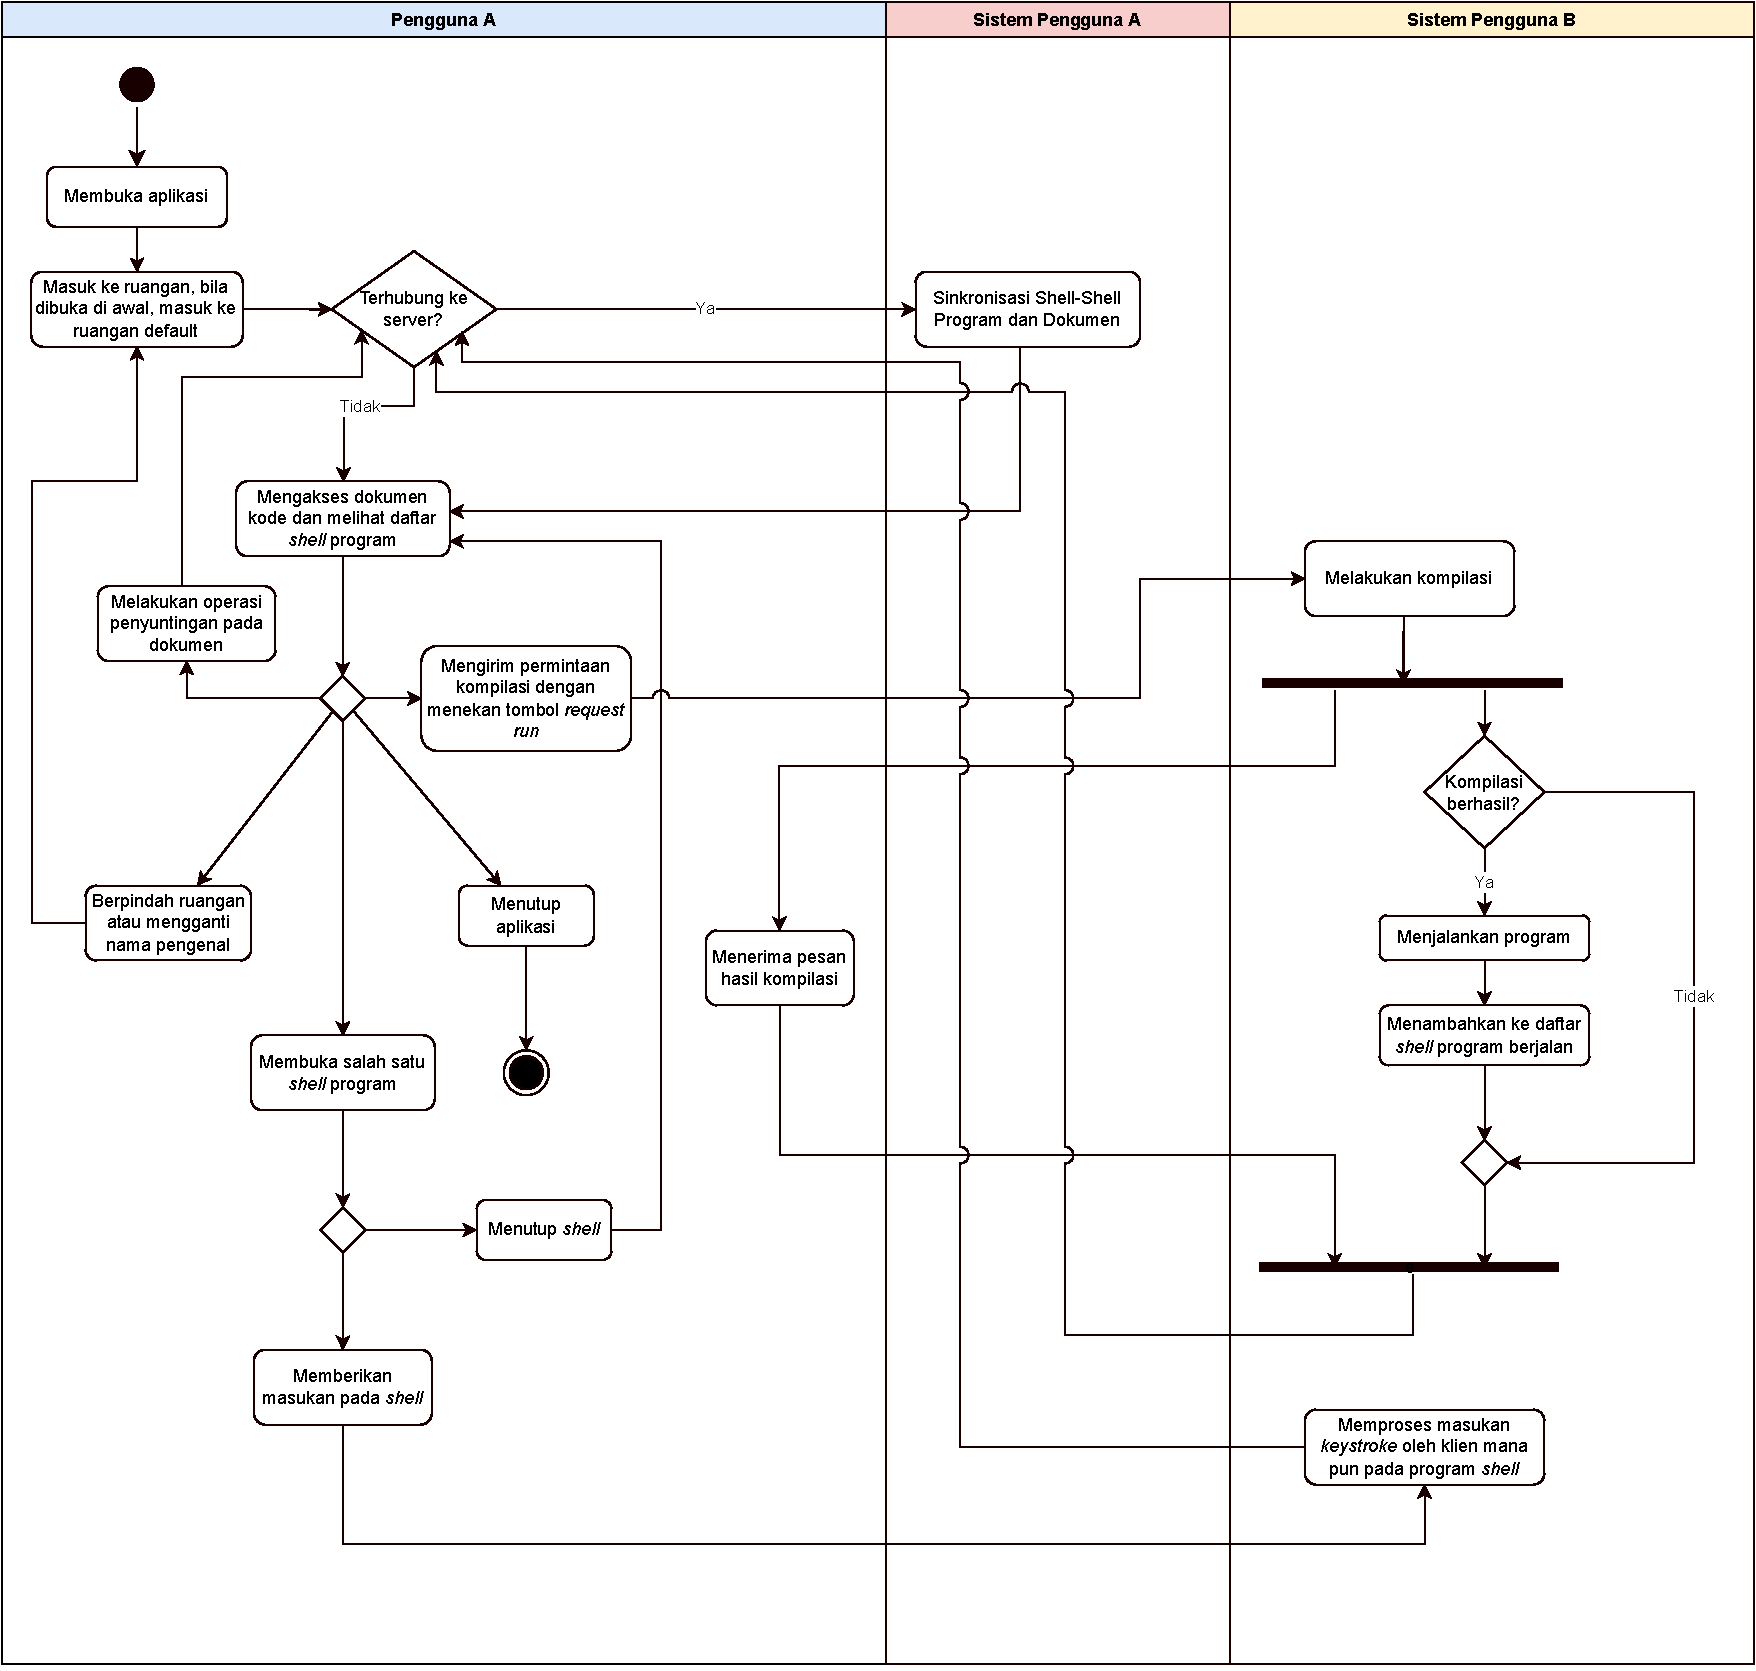
\includegraphics[scale=0.5]{assets/skripsi/Activity_Diagram}
    \caption{\textit{Activity Diagram} Alur Penggunaan Secara \textit{High Level}}
    \label{fig:activity}
\end{figure}

Pada Gambar~\ref{fig:activity}, perilaku sinkronisasi \textit{shell-shell} program dan dokumen dilakukan tergantung dengan variasi implementasi dari program. Pada arsitektur \textit{client-server}, sistem aplikasi pengguna A akan berhubungan dan melakukan sinkronisasi dengan server. Sementara pada arsitektur \textit{peer-to-peer}, sistem aplikasi pengguna A akan berhubungan langsung dan melakukan sinkronisasi dengan \textit{peer} atau klien lain. Selain itu, permintaan dan transmisi pesan hasil kompilasi dilakukan melalui pengiriman pesan secara langsung pada arsitektur \textit{peer-to-peer}, namun harus melalui perantara server pada arsitektur \textit{client-server}. Detail implementasi dan arsitektur detail aplikasi akan dirincikan pada Bab~\ref{bab:4} Implementasi. Sistem yang telah dikembangkan kemudian akan dilakukan evaluasi secara objektif berdasarkan aspek-aspek tertentu yang menrepresentasikan performa dan skalabilitas aplikasi.

\section{Aplikasi dan \textit{Framework} Terkait}

Terdapat beberapa aplikasi dan \textit{library} yang terkait dalam pengembangan sistem aplikasi PeerToCP yang dibahas dalam penelitian ini. Berbagai \textit{framework}, \textit{library}, dan sistem modul ini merupakan hasil penelitian oleh para pengembang sebelumnya.

\subsection{Electron}

Electron merupakan salah satu \textit{framework} aplikasi desktop yang melibatkan HTML, CSS, dan JavaScript. Bagian belakang atau \textit{backend} dari Electron berjalan dengan lingkungan \textit{runtime} Node.js. Node.js merupakan bahasa yang menggunakan \textit{syntax} yang serupa dengan Javascript dan dapat dikompilasi melalui kopmilator yang disebut V8 engine. Bagian tampilan atau \textit{frontend} dari Electron memanfaatkan aplikasi \textit{Chromium} yang dapat mengolah bahasa \textit{markup} web, seperti HTML (\textit{HyperText Markup Language}), CSS (\textit{Cascading Style Sheets}), serta JavaScript.

Salah satu keuntungan menggunakan Electron adalah aplikasinya yang bersifat \textit{cross-platform} atau dapat berjalan di beragam sistem operasi, seperti Windows, GNU/Linux, atau MacOS. Keuntungan lainnya ialah karena bersifat aplikasi desktop, Electron dapat mengakses berbagai macam fungsi antar muka sistem operasi, seperti memanggil subproses pada kernel dan menulis berkas. Karena \textit{frontend}-nya yang menggunakan bahasa web pula, aplikasi yang dibuat dengan Electron cenderung lebih mudah untuk dipindahkan dan diadaptasi dengan fungsi terbatas pada web.

\subsection{Yjs}

Yjs merupakan sebuah \textit{framework} library yang mengimplementasi CRDT yang disebut dengan YATA (\textit{Yet Another Transformation Approach})~\citep{Nicolaescu2016yjs}.

\subsubsection{y-docs}

\subsubsection{y-protocols}

\subsubsection{y-websocket}

\subsubsection{y-webrtc}

\subsection{Codemirror}

Codemirror merupakan komponen \textit{frontend} editor kode yang dapat diolah oleh peramban web. Codemirror menyediakan banyak ekstensi, aksesibilitas tinggi, serta dukungan untuk berbagai macam bahasa pemrograman. Codemirror berguna untuk menampilkan editor kode dan memiliki ekstensi yang menghubungkannya dengan Yjs dan sudah diuji oleh pengembang Codemirror.

\subsection{Xterm.js}

Xterm.js merupakan salah satu komponen \textit{frontend} yang menampilkan terminal melalui bahasa yang dapat diolah oleh web. Xterm.js memiliki antarmuka yang bisa menerima dan meneruskan data dari peramban (\textit{browser}) yang dapat dihubungkan dengan sebuah proses berjalan pada kernel. Xterm.js dikembangkan tanpa memerlukan dependensi, sehingga cocok digunakan untuk pengembangan sistem yang membutuhkan tampilan \textit{shell} secara instan.

\subsection{Node-pty}

Node-pty merupakan \textit{library} Node.js yang memberikan antarmuka untuk melakukan \textit{fork} proses dengan deskriptor berkas \textit{pseudoterminal}. Node-pty mengizinkan adanya aliran data untuk baca dan tulis dengan proses berjalan pada kernel. Node-pty berguna untuk menjalankan berkas hasil kompilasi yang bersifat CLI (\textit{Command Line Interface}) yang tidak memiliki tampilan grafik untuk pengguna. Node-pty juga bersifat \textit{cross-platform} mendukung sistem operasi Windows, GNU/Linux, dan MacOS.


\subsection{Kode dan Kompilasi}

Proses kompilasi merupakan proses mengonversi kode dari bahasa dengan level yang lebih tinggi dan dapat dimengerti oleh manusia menjadi kode biner yang dapat dimengerti oleh mesin. Pada penelitian ini, selain editor kode yang bersifat kolaboratif, proses kompilasi kode tunggal juga hendaknya dapat dilakukan oleh salah satu pengguna. Proses kompilasi ini membutuhkan kompilator yang terpasang pada suatu sistem operasi.

\section{Tampilan Antarmuka dan Interaksi Aplikasi dengan Pengguna}

Disini akan dijelaskan cara menggunakan aplikasi

\section{Arsitektur Peer-To-Peer}

\begin{figure}
    \centering
    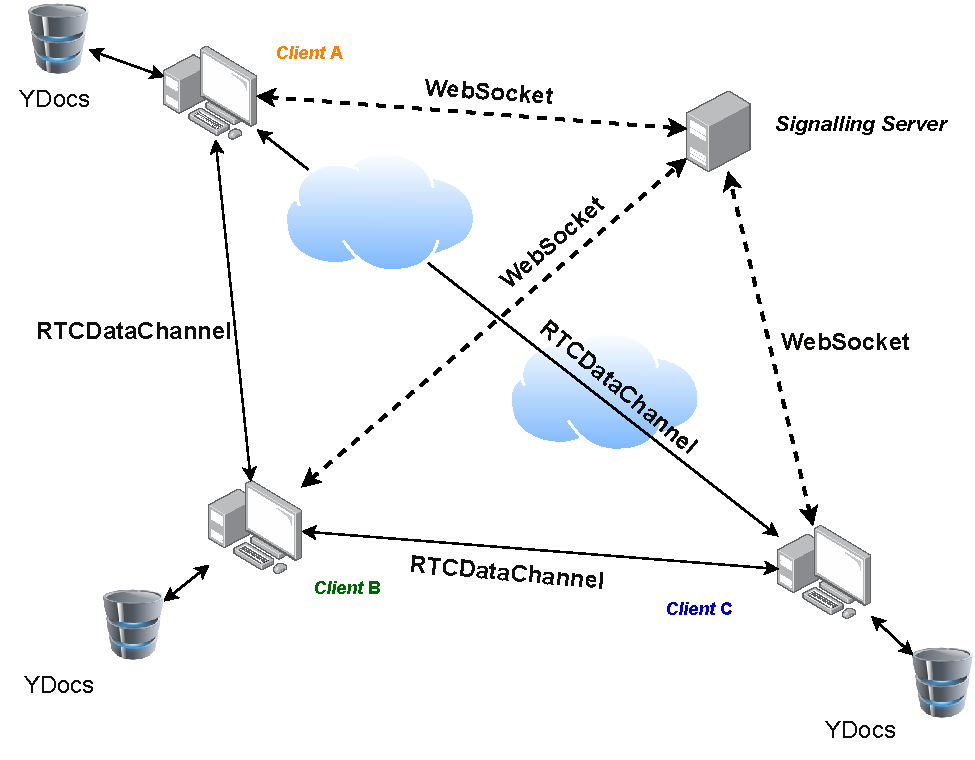
\includegraphics[scale=0.6]{assets/skripsi/Arsitektur_WebRTC_CRDT}
    \caption{Arsitektur WebRTC-CRDT}
\end{figure}

\section{Arsitektur Client-Server}

\begin{figure}
    \centering
    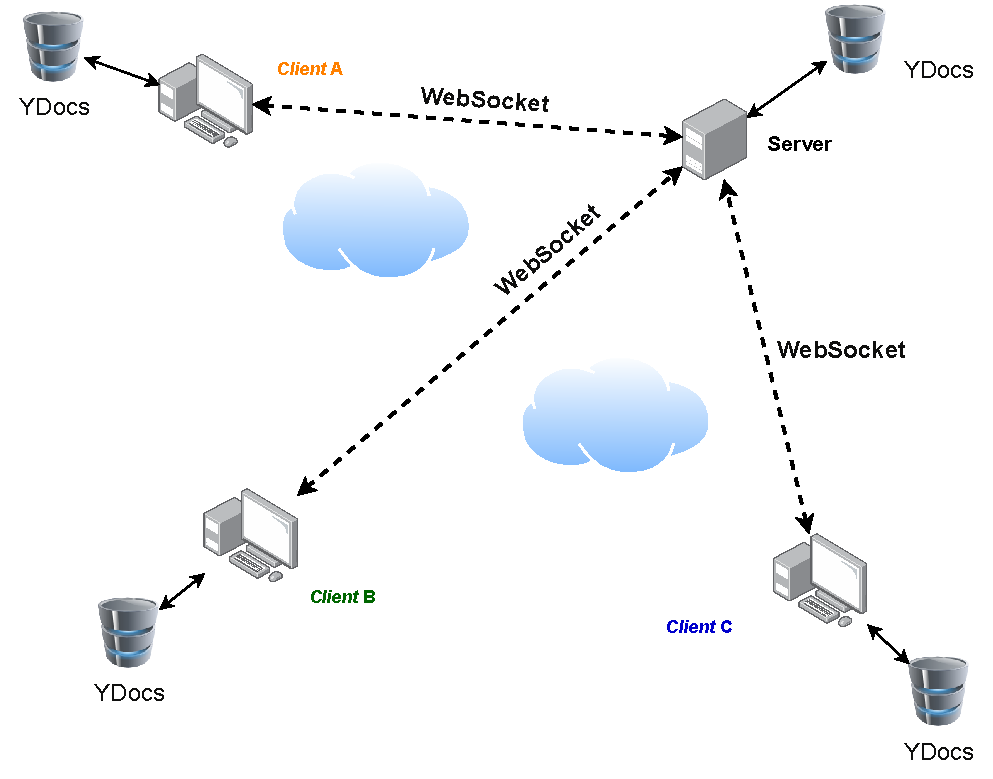
\includegraphics[scale=0.42]{assets/skripsi/Arsitektur_WebSocket_CRDT}
    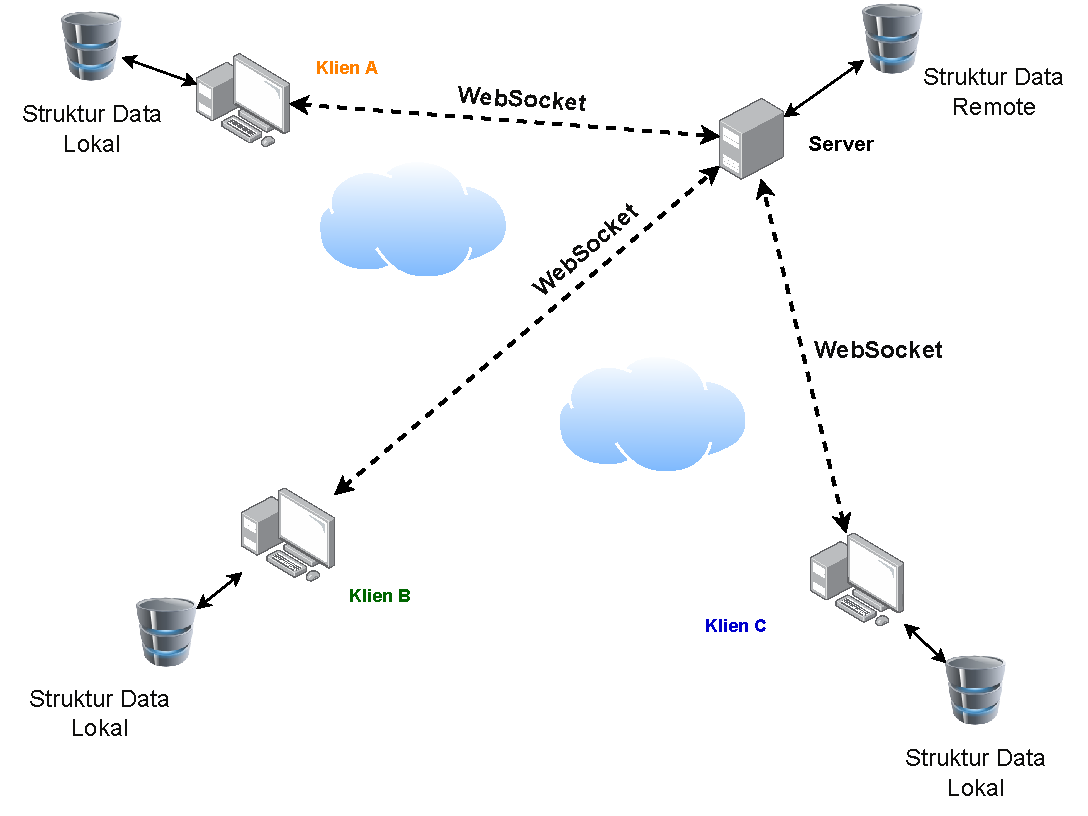
\includegraphics[scale=0.42]{assets/skripsi/Arsitektur_WebSocket_OT}
    \caption{Arsitektur WebSocket-CRDT dan WebSocket-OT Secara Berurutan}
\end{figure}

